\documentclass[11pt roman]{article}

%Change the font style of the document
 %\renewcommand{\familydefault}{\ttdefault}
 
 %\usepackage{indentfirst} %auto add indent to new paragraphs
 \usepackage{graphicx} %package for image handling
 \usepackage{float} %package for image handling. keep in place exactly in code
 
 
\begin{document}

%create the title page=================

\title{ECE 650 - Final Course Project}
\author{BY: Brian Luong, Shanthi Meena Arumugam}
\date{2022-04-08}
%\maketitle
\begin{titlepage}
    \vspace*{\fill}
    \begin{center}
	  \begin{huge} 
	  ECE 650 - Final Course Project \\
	  \end{huge}
	  
	  BY: Brian Luong, Shanthi Meena Arumugam\\
      2022-04-08
    \end{center}
    \vspace*{\fill}
\end{titlepage}

%=======================================
\pagebreak


\section{Introduction}
This report focuses on solving the minimum vertex cover of an undirected graph which is an example of an NP-complete problem. The minimum vertex cover is a set of vertices where every edge of the graph is incident to at least one of the vertex found in the cover - in other words, given graph $G=(V,E)$ the cover $C \subseteq V$ such that each edge $E$ is incident to at least one vertex in $C$. \\\\

In the proceeding sections, the run time and approximation ratio will be discussed with respect to the input graph size and the three methods used to solve such problem.
\section{Methods}
The three methods used in this project are as followed:\\\\

\emph{CNF-SAT}- A polynomial time reduction of the problem to turn the Vertex-Cover problem into a CNF satisfiability problem. In our case, given a graph $G, $and$ k$, a CNF formula can be generated and fed into a SAT solver (minisat).\\\\  

\emph{APPROX-1}- A systematic approach to solve the minimum vertex cover problem. Given a graph, choose the highest degree (most incident edges) vertex and add it to the cover. Update all incident edges on that vertex. Repeat until all edges are covered.\\\\

\emph{APPROX-2}- Another systematic approach. Pick an edge from the graph and add the two vertices to the cover. Throw away all edges attached to the two vertices. Repeat until all edges are covered. This is similar to APPROX-1 but instead of looking for the highest degree vertex, we choose any edge.

\section{Setup}
The inputs used for this project were created using the graphGen program found on eceubuntu (/home/agurfink/ece650/graphGen/grahGen). This generator takes the number of desired vertices as its only input and generates $V..$ and $E \{<...>,...\}$ statements. The $V$ statement indicates how many vertices are found in the graph and $E$ indicate the edges of the graph. \\\\

With this program, the inputs for graphs with sizes ranging from 5 to 50 (in steps of 5) vertices can be created and passed into the project for processing. The output of the project program is the vertex cover itself, the runtime for each method and the approximation ratio. After collecting 10 runs of each graph size, the following data was graphed. It should also be noted that the project program will time-out its method calculation if it takes longer than 2 seconds to complete.
\section{Analysis}
\graphicspath{ {../} } %relative path to where photos are


We calculated the running time and approximation ratio for each strategy to see how efficient it is. For each value of V (V= 5,10,15,20...,45,50), we created 10 graphs, ran the software 10 times for each graph, and calculated the mean and standard deviation across those 100 runs for each value of V. Following that, we'll look at the experimental outcomes from two perspectives: \\

\subsection{ Running Time:}
We calculated the average and standard variance of each algorithm thread's running duration. Because CNF-SAT takes much longer to run than the preceding two algorithms, we generate the graphs individually. The running times of APPROX-1 and APPROX-2, as well as CNF-SAT, are shown RunningTimeOfCNF-SAT and RunningTimeOfVC1AndVC2 images, where the x-axis represents the number of vertices and the y-axis represents the running time (ms).\\

Because of the temporal complexity, both the APPROX-1 and APPROX-2 grow with an increasing n vertices, as seen in RunningTimeOfVC1AndVC2 image. When comparing the two approaches, APPROX-1 takes longer to run since it requires more sequential loops and computations in our program to select the vertex with the highest degree, whereas APPROX-2 simply selects the edge at random. \\


When the graph contains a large number of vertices and edges, the CNF-SAT algorithm takes substantially longer to run. During the experiment, we discovered that trying to run a programme that accepts a graph with 20 or more vertices takes an excessively long time, which is why they aren't represented in RunningTimeOfCNF-SAT image. It shows that as the number of vertices increases, the running time increases exponentially. This is due to the fact that it is an NP-complete problem that cannot be solved in polynomial time. 

\begin{figure}[H]
	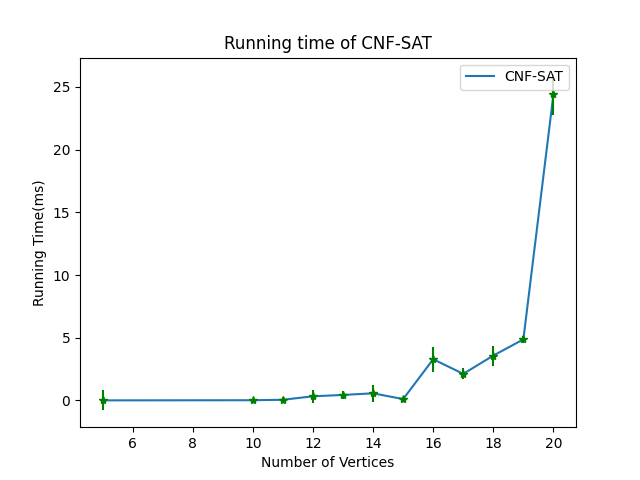
\includegraphics[scale=0.6]{RunningTimeOf_CNF-SAT_}\\ %png name
	\centering
	\caption{Runtime of CNF-SAT method up to 20 vertices. Runs 20 and above resulted in CNF-SAT time-out}
\end{figure}


\begin{figure}[H]
	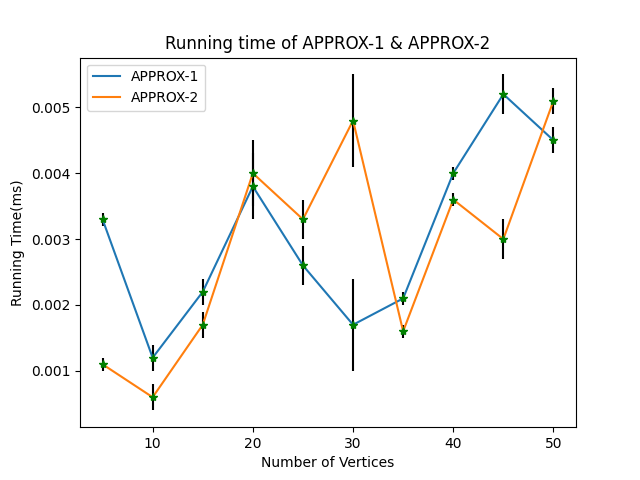
\includegraphics[scale=0.6]{RunningTimeOf_VC1_And_VC2_}\\ %png name	
	\centering
	\caption{Runtime of APPROX-1 and APPROX-2 up to 50 vertices.}
\end{figure}


\subsection{ Approximation Ratio:}
We calculated the APPROX-1 and APPROX-2 approximation ratios, which are the ratios of the estimated vertex cover size to the size of an optimal (minimum-sizes) vertex cover. The approximation ratio of APPROX-1 and APPROX-2 is shown in APROXIMATIONRATIO image, with the x-axis reflecting the number of vertices and the y-axis representing the approximation ratio. V=5,10,15 are used to create the graphs.

\begin{figure}[H]%big h to force placement
	\includegraphics[scale=0.6]{APROXIMATION_RATIO}\\ %png name
	\centering
	\caption{Approximation ratio of the three methods up to 20 vertices. Runs 20 and above resulted in CNF-SAT time-out}
\end{figure}

As seen in APROXIMATIONRATIO image, APPROX-VC-1 generates a result that is close (essentially 1:1) to the optimal (minimum-sizes) solution, however, APPROX-2 produces a greater vertex cover, implying that it cannot ensure the correctness of minimum-sizes findings.

When the data scale is small, the efficiency of the CNF-SAT approach is the greatest of all for finding minimum vertex cover; however, if there are more vertices and edges, the running time would considerably increase compared to the other two approaches, making it difficult to achieve. Although APPROX-2 takes the shortest time to run, the approximation ratio indicates that it cannot always calculate the lowest vertex cover accurately. APPROX-1 also has a considerably shorter runtime and performs well in terms of approximation ratio, which is quite close to the ideal findings, therefore it can be considered a more efficient solution as data grows larger.



\section{Conclusion}
The implementation of three various approaches to the vertex cover problem is first shown in this report, followed by a study of each method's efficiency in terms of running time and approximation ratio, and finally, an overall comparison for each of them under various scenarios.

\newpage\section{References}
[1] https://git.uwaterloo.ca/ece650-1221/pdfs/-/blob/master/uw-ece650-1221-prj.pdf 
[2] Advanced Linux Programming, Mark Mitchell, Jeffrey Oldham, and Alex Samuel



\end{document}


